\documentclass{beamer}


\usepackage{mjclectureslides}

\renewcommand*{\thefootnote}{\fnsymbol{footnote}}

\definecolor{Dblue}{rgb}{.255,.41,.884}

\title[Random variables]{Introduction to Probability \\ Random variables}
%\author[Prof. Michael Carlisle]{Prof. Michael Carlisle}
%\institute{Baruch College, CUNY}
%\date{Spring 2018}
\date{}

\begin{document}

\frame{\titlepage}


\frame{ \frametitle{Random variables (RVs)}

A \textbf{random variable} is a function which takes an outcome from a sample space as input, and outputs a real number: 
\[ X: \Omega \to \R. \]
(Think: this looks just like a function $g:D \to \R$.)

\vspace{5mm}

We can talk about random variables taking certain values as events that have probabilities. 

\vspace{5mm}

If $\omega \in \Omega$, $X(\omega)$ (like $g(x)$) is the value of $X$ given by outcome $\omega$. 

\vspace{5mm}

The set of possible values of $X$ is called the \textbf{range} or \textbf{image} of $X$ (and we denote it $R_X$ or $X(\Omega)$, like the image $f(D)$).

}


\frame{ \frametitle{Random variables (RVs) (discrete)}

A random variable whose range is finite or countable is called a \textbf{discrete random variable}.

\vspace{5mm}

\begin{ex}
Let $\Omega$ be the sample space of sequences of 4 coin flips, and define $X$ to be the function giving the number of H in a sequence. 
\end{ex}

Some values $X$ takes: 

\begin{itemize}
\item $X(HHHH) = 4$, $X(TTTT) = 0$
\item $X(THTT) = 1$, $X(HTTH) = 2$
\end{itemize}
You should be able to see from these examples that $X$ can take five different values: $X(\omega) \in X(\Omega) = \{0, 1, 2, 3, 4\}$. 

}


\frame{ \frametitle{RV Events, Probability mass function (PMF)}

Now we can ask questions about experiments based on the values of RVs that use outcomes to generate numbers. 

\vspace{5mm}

For our 4-flip example, we can ask, for example, 

\vspace{5mm}

\begin{center}
``What is the probability that $X = 3$''?
\end{center}

}


\frame{ \frametitle{RV Events, Probability mass function (PMF)}

The event $E = \{X = 3\}$ is a set of outcomes: 
\[ \{X = 3\} = \{ \omega \in \Omega: \, X(\omega) = 3\} = \{HHHT, HHTH, HTHH, THHH\}. \]
This type of set is called a \textbf{pre-image}, and its notation is 
\[ X^{-1}(3) = \{X = 3\}. \] 
Its probability is written without the brackets: $P(E) = P(X = 3)$. 

}


\frame{ \frametitle{Probability mass function (PMF)}

The \textbf{probability mass function (PMF)}, or more simply, \textbf{probability function}, is a function that gives the probability of the event of a single value a random variable $X$ can take. 

\vspace{3mm}

\begin{ex}
$p_X: \mathbb{R} \to \mathbb{R}$ is the PMF of a random variable $X$ that gives the number of H from 4 fair coin flips. 
\[ p_X(i) = \left\{ \begin{array}{ll}
\frac{1}{16} & i = 0, 4 \\
\frac{4}{16} & i = 1, 3 \\
\frac{6}{16} & i = 2 \\
0 & i \not \in X(\Omega) = \{0, 1, 2, 3, 4\}
\end{array}\right. \]
\end{ex}

We can graph a PMF on a \textbf{histogram} (bar chart). 

}


\frame{ \frametitle{Properties of a PMF}

For a PMF $p_X$ of any discrete random variable $X$, the following properties hold: 

\begin{itemize}
\item \textbf{(nonnegativity)} $0 \leq p_X(i) \leq 1$ for any $i \in \mathbb{R}$
\item \textbf{(value only on range of $X$)} $p_X(i) = 0$ if $i \not \in X(\Omega)$
\item \textbf{(normalization)} $\sum_{i \in X(\Omega)} p_X(i) = 1$. 
\end{itemize}

\vspace{3mm}

We also call the PMF $p_X$ the \textbf{distribution} of $X$. 

}


\frame{ \frametitle{Uniform PMF}

A \textbf{uniform random variable} on the set of values 
\[ A = \{a_1, a_2, ..., a_n\} \] 
is like rolling an $n$-sided die, each face of which has a different value $a_i$ on it. 

\vspace{5mm}

If $Y$ is a uniform random variable on this set $A$, its PMF is 
\[ p_Y(x) = \left\{ \begin{array}{ll} \frac{1}{n} & \text{ if } x \in A \\ 0 & \text{ if } x \not \in A. \end{array}\right. \]

\vspace{5mm}

The most common example of a uniform random variable is a die roll itself: a six-sided die takes values on $\{1, 2, 3, 4, 5, 6\}$ each with probability $\frac{1}{6}$. 

}


\frame{ \frametitle{Bernoulli random variables}

$X$ is called a \textbf{Bernoulli random variable} \emph{with parameter } $p$ (written Bern($p$)) if its PMF is 
\[ p_X(1) = p, \, p_X(0) = 1-p. \]
This is the RV of a (biased) coin that flips 1 on H with probability $p$ and 0 on T.

\vspace{2mm}

\begin{ex}
``Roll a 5 on a die'' has success probability $\frac{1}{6}$, and so failure probability $\frac{5}{6}$. Thus, for $X \sim$ Bern($\frac{1}{6}$), the probability you roll a 5 is 
\[ p_X(1) = \frac{1}{6}. \]
\end{ex}

}


\frame{ \frametitle{Binomial random variables}

$X$ is called a \textbf{binomial random variable} \emph{with parameters } $n$, $p$ (written Bin($n$, $p$)) if its PMF is 
\[ p_X(k) = {n \choose k} p^k (1-p)^{n-k}, \, k=0,1,2,...,n. \]
This is the RV that adds up $n$ Bernoulli RVs above: if $X_1, X_2$, ..., $X_n$ are IID Bern($p$), then $X = \sum_{i=1}^n X_i \sim Bin(n,p)$. 

\vspace{2mm}

\begin{ex}
``Roll a 5 on a die'' has success probability $\frac{1}{6}$, and so failure probability $\frac{5}{6}$. Thus, for $X \sim$ Bin(7, $\frac{1}{6}$), the probability you roll a 5 exactly three times out of seven is 
\[ p_X(3) = {7 \choose 3} \left(\frac{1}{6}\right)^3 \left(\frac{5}{6}\right)^4. \]
\end{ex}

}


\frame{ \frametitle{Geometric random variables}

$X$ is called a \textbf{geometric random variable} \emph{with parameter } $p$ (written Geom($p$)) if its PMF is 
\[ p_X(k) = p(1-p)^{k-1}, \, k = 1, 2, ....\]
This RV represents the number of trials up to a ``success'' in a run of repeated IID experiments with ``success'' probability $p$. That is, $k-1$ ``failures'', and then ``success'' on trial $k$. 

\vspace{2mm}

\begin{ex}
``Roll a 5 on a die'' has success probability $\frac{1}{6}$, and so failure probability $\frac{5}{6}$. Thus, for $X \sim$ Geom($\frac{1}{6}$), the probability it takes exactly 4 rolls to get the first 5 is 
\[ p_X(4) = \left(\frac{1}{6}\right) \left(\frac{5}{6}\right)^3. \]
\end{ex}

}


\frame{ \frametitle{Pascal (negative binomial) random variables}

$X$ is called a \textbf{Pascal} (or \textbf{negative binomial}) \textbf{random variable} with parameters $(m, p)$ (written NB($m, p$)) if, generalizing the geometric, represents the $m$th success (with probability $p$) on the $k$th trial of repeated IID experiments (that is, $k-m$ failures, $m$ successes, with trial $k$ being the $m$th success). Its PMF is 
\[ p_X(k) = { k-1 \choose m-1} p^m (1-p)^{k-m}, \, k = m, m+1, m+2, .... \]

\vspace{2mm}

\begin{ex}
``Roll a 5 on a die'' has success probability $\frac{1}{6}$, and so failure probability $\frac{5}{6}$. Thus, for $X \sim$ NB(4, $\frac{1}{6}$), the probability it takes 10 rolls to get the fourth 5 is 
\[ p_X(10) = { 10-1 \choose 4-1} p^{4} (1-p)^{10-4} = {9 \choose 3} \left(\frac{1}{6}\right)^4 \left(\frac{5}{6}\right)^6. \]
\end{ex}

}



\frame{ \frametitle{Poisson random variables}

$X$ is called a \textbf{Poisson} \textbf{random variable} with parameter $\lambda$ (written Poisson($\lambda$)) if the PMF of $X$ is 
\[ p_X(k) = e^{-\lambda} \frac{\lambda^k}{k!}, \, k = 0, 1, 2,3, .... \]
This counts the number of ``rare events'' with ``average'' rate of occurrence $\lambda$.

\vspace{5mm}

We can use a Poisson($\lambda$) to approximate a Bin($n,p$), using $\lambda = np$, if the number of trials $n$ is ``large'' and success probability $p$ is ``small''.\footnote{We'll revisit this fact in the next set.}

}


\frame{ \frametitle{Poisson random variables: approximate lottery win}

``Win the New York Lottery game Win 4 Straight Play with a \$1 ticket'' has success probability $p = 0.0001$. 

\vspace{5mm}

Thus, for a Poisson($\lambda = 0.02$), which would simulate buying $n=200$ tickets, so that $\lambda = np = 200(0.0001) = 0.02$, the probability you hold at least one winning ticket is 
\begin{align*}
P(X \geq 1) = 1 - P(X = 0) & = 1 - p_X(0) \\
 & = 1 - e^{-0.02} \frac{0.02^0}{0!} \\
 & = 1 - e^{-0.02} \approx 0.0198,
\end{align*}
about 1.98\%. 

}


\frame{ \frametitle{Hypergeometric random variables}

$X$ is called a \textbf{hypergeometric} \textbf{random variable} with parameters $r$, $n$, $N$ if the PMF of $X$ is 
\[ p_X(k) = \frac{ {r \choose k} {N-r \choose n-k} }{ {N \choose n} }, \, k = 0, 1, 2, ..., n. \]
Consider an urn with $N$ balls: $r$ are red and $N-r$ are green. \\
$X$ counts the number $k$ of red balls (and $n-k$ green) drawn if the experiment is to draw $n$ balls without replacement (i.e. all at once). 

%\onslide<2->
\vspace{2mm}

\begin{ex}
Say there are $N = 20$ balls in the urn: $r = 8$ red and $N-r = 12$ green. If you draw $n = 6$ of them without replacement, what is the probability you get 5 red (and so only 1 green)?
\[ p_X(5) = \frac{ {8 \choose 5} {12 \choose 1} }{ {20 \choose 6} } = \frac{28}{1615} \approx 0.017337. \]
\end{ex}

}



\frame{ \frametitle{Cumulative distribution function (CDF)}

The \textbf{cumulative distribution function (CDF)} of a discrete random variable $X$ is the sum of all the probabilities below a certain value. 

\vspace{5mm}

If $p_X$ is the PMF of a random variable $X$, then the CDF of $X$ is 

\[ F_X: \mathbb{R} \to \mathbb{R}, \,\, F_X(a) = P(X \leq a) = \sum_{i \leq a, \,\, i \in X(\Omega)} p_X(i). \]

}


\frame{ \frametitle{Properties of a CDF}

\begin{itemize}
\item $\lim_{a \to -\infty} F_X(a) = 0$ and $\lim_{a \to \infty} F_X(a) = 1$.
\item $F_X$ is a nondecreasing function: if $a \leq b$, then $F_X(a) \leq F_X(b)$. 
\item For $X$ a discrete RV, at each value $X = i$ takes with nonzero probability, $F_X$ jumps up by $p_X(i)$. 
\end{itemize}

%%\onslide<2->

\begin{ex}
$p_X: \mathbb{R} \to \mathbb{R}$ is the PMF of a random variable $X$ that gives the number of H from 4 fair coin flips. Then the CDF of $X$ is 
\[ F_X(a) = \left\{ \begin{array}{ll}
0 & a < 0 \\
\frac{1}{16} & 0 \leq a < 1 \\
\frac{1}{16} + \frac{4}{16} = \frac{5}{16} & 1 \leq a < 2 \\
\frac{5}{16} + \frac{6}{16} = \frac{11}{16} & 2 \leq a < 3 \\
\frac{11}{16} + \frac{4}{16} = \frac{15}{16} & 3 \leq a < 4 \\
1 & a \geq 4
\end{array}\right. \]
\end{ex}

}


\frame{ \frametitle{Continuous Function Review: Integration} 

Recall, the \textbf{indefinite integral}, or \textbf{antiderivative}, of the function $y=f(x)$, is denoted 
\[ \int f(x) dx = F(x) + C, \]
where $C$ is any constant. $F(x) + C$ is a family of functions, differing only by the \textbf{constant of integration}. 

}


\frame{ \frametitle{Continuous Function Review: Integration} 

The \textbf{definite integral} of $f(x)$, over the integral $(a,b]$, is the (signed) area between the curve and the $x$-axis, which is calculated by a difference of the antiderivative $F(x)$ evaluated at the endpoints of the interval (the \textbf{limits of integration}), $a$ and $b$: 
\[ \int_a^b f(x) dx = (F(b) + C) - (F(a) + C) = F(b) - F(a). \]


}



\frame{ \frametitle{Improper integration}

An \textbf{improper integral} is a definite integral where at least one of the limits of integration is infinite (i.e. $a = -\infty$ or $b = \infty$ or both), or the function $y=f(x)$ goes to $\infty$ or $-\infty$ somewhere during the interval of integration (this second kind is also called \textbf{singular}). 

\vspace{3mm}

\[ \textbf{Example: } \,\, \int_{0}^{\infty} f(x) dx \text{ is an improper integral.} \]

\vspace{3mm}

(We will not discuss improper integrals, but not singular integrals.)


}



\frame{ \frametitle{Continuous random variables}

A \textbf{continuous random variable} is a random variable $X: \Omega \to \R$ which varies continuously with changes in the sample space input. 

\vspace{5mm}

For discrete random variables, we used sums to describe probabilities and functions, such as expected value and variance, that describe properties of a random variable. 

\vspace{5mm}

For continuous random variables, we will use integrals to do this.

}


\frame{ \frametitle{Probability Density Function (PDF)}

The \textbf{probability density function (PDF)} of a continuous random variable $X$ takes the place of the probability mass function (PMF) of a discrete random variable. 

\vspace{3mm}

We call a real-valued function $f(x)$ a \textbf{probability density function (PDF)} of some continuous RV $X$ if $f$ satisfies the following: 

\begin{itemize}
\item $f(x) \geq 0$ for all $x \in \R$
\item $\int_{-\infty}^{\infty} f(t) dt = 1$
\end{itemize}

If $f$ is the PDF of $X$, then we can find the probability of $X$ being in the interval $(a,b]$ by 
\[ P(X \in (a,b]) = P(a < X \leq b) = \int_a^b f(t) dt. \]

}


\frame{ \frametitle{Continuous RV: cumulative distribution (CDF)}

The \textbf{cumulative distribution function (CDF)} of a continuous random variable $X$ takes the same place as for a discrete random variable.

\vspace{3mm}

We call a real-valued function $F(x)$ a \textbf{cumulative distribution function (CDF)} of some continuous RV $X$ if $\exists$ a PDF $f$ such that 
\[ F(x) = P(X \leq x) = \int_{-\infty}^{x} f(t) dt. \]

}


\frame{ \frametitle{Continuous RV: cumulative distribution (CDF)}

$F$ has several properties: 
\begin{itemize}
\item $\lim_{a \to -\infty} F_X(a) = 0$ and $\lim_{a \to \infty} F_X(a) = 1$.
\item $F_X$ is a nondecreasing function: if $a \leq b$, then $F_X(a) \leq F_X(b)$. 
\item $F$ is continuous on all of $\R$ (no jumps)
\item $P(a < X \leq b) = \int_a^b f(t) dt = F(b) - F(a)$
\end{itemize}

}


\frame{ \frametitle{Continuous RV: $X$ has no point masses}

In this last property, note that since $F$ is continuous, computed from an integral, we have the property that $X$ has no point masses: thus, 
\[ P(a < X \leq b) = P(a \leq X < b) = P(a < X < b) = P(a \leq X \leq b), \]
and so 
\[ P(X = c) = \int_c^c f(t) dt = 0 \text{ for any } c \in \R. \] 

We can, however, compute $P(X \approx a)$ if we clarify the question.

}


\frame{ \frametitle{Continuous RV: infinitesimal approximation}

Let $a \in \R$ and $\varepsilon > 0$ be a small distance. The probability that $X$ with PDF $f$ is ``very close to $a$'' (i.e. $P(X \approx a)$) can be calculated in one way\footnote{There are other ways, of course.} by  
\[ P(X \approx a) \approx P(a < X \leq a + \ve) = \int_{a}^{a + \ve} f(x) dx. \]

}


\frame{ \frametitle{Continuous RV: infinitesimal approximation}

If you wish to avoid computing the integral, recall the definition of the derivative, and how to relate the CDF to the PDF: 
\begin{align*}
f(a) = F'(a) = \lim_{\ve \to 0} \frac{F(a + \ve) - F(a)}{\ve} = \lim_{\ve \to 0} \frac{\int_{a}^{a + \ve} f(x) dx}{\ve}.
\end{align*}
Thus, noting that the PDF $f$ is \emph{not} a probability itself, but a function used to compute probabilities, we can approximate 
\[ P(X \approx a) \approx \ve \cdot f(a). \]

}


\frame{ \frametitle{Indicator functions, random variables}

Many continuous random variables only take values on some of the real number line; it is useful to use \textbf{indicator functions} to make writing down PDFs easier. 

\vspace{5mm}

The \textbf{indicator function} on the set $A$ is defined by 
\[ 1_{A}(x) = \left\{ \begin{array}{cl} 1 & x \in A \\ 0 & x \not \in A. \end{array} \right. \]
When part of a PDF, indicators indicate the \textbf{support} (nonzero domain) of the PDF. (Sometimes the notation is $I_A(x)$.)

\vspace{5mm}

A continuous random variable with PDF consisting \emph{solely} of an indicator function is called an \textbf{indicator random variable}, which indicates a ``success'' of a trial if the outcome $\omega \in A$. 

}


\frame{ \frametitle{Uniform random variables}

One of the simplest continuous RV is the \textbf{uniform} random variable, which moves the notion of ``equally likely'' from a discrete set of values to an entire interval on the real line. 

\vspace{5mm}

$X$ is a uniform random variable on the interval $(a,b)$, denoted $X \sim Unif(a,b)$, if it has PDF 
\[ f(x) = \frac{1}{b-a}1_{(a,b)}(x). \]

\vspace{5mm}

If $X \sim Unif(a,b)$, then its CDF is given by 
\[ F(x) = P(X \leq x) = \int_{-\infty}^{x} 1_{(a,b)}(t) dt = \left\{ 
\begin{array}{cl}
0 & x \leq a \\
\frac{x-a}{b-a} & a < x < b \\
1 & x \geq b.
\end{array}
\right. \]

}


\frame{ \frametitle{Exponential random variables}

An \textbf{exponential} random variable models the amount of time it takes for a given impending event to occur as exponential decay. $X \sim Exp(\lambda)$ has PDF 
\[ f(x) = \lambda e^{-\lambda x} 1_{(0,\infty)}(x). \]

\vspace{5mm}

If $X \sim Exp(\lambda)$, then its CDF is given by 
\[ F(x) = P(X \leq x) = \int_{-\infty}^{x} \lambda e^{-\lambda t} 1_{(0,\infty)}(t) dt = \left\{ 
\begin{array}{cl}
0 & x \leq 0 \\
1 - e^{-\lambda x} & x > 0.
\end{array}
\right. \]

}


\frame{ \frametitle{Gamma random variables}

Exponential random variables are a special case of \textbf{Gamma} random variables. 

\vspace{3mm}

$X \sim Gamma(\alpha, \beta)$ (with $\alpha$ the ``rate'' parameter and $\beta$ the ``shape'' parameter) if its PDF is 
\[ f(x) = \frac{\alpha(\alpha x)^{\beta - 1} e^{-\alpha x}}{\Gamma(\beta)} 1_{(0,\infty)}(x), \]
where the \textbf{Gamma function} is $\Gamma(x) = \int_{0}^{\infty} t^x e^{-t} dt$, which is the general form of factorial: $\Gamma(n) = (n-1)!$ for $n \in \N$. 

\vspace{5mm}

$Exp(\lambda) \sim Gamma(\lambda, 1)$, and for $n \in \N$, a $Gamma(\lambda, n)$ RV models the sum of $n$ IID $Exp(\lambda)$ (counts the total time for $n$ consecutive events of the same type to occur). 

}



\frame{ \frametitle{Normal random variables}

\textbf{Normal} random variables are used to model vast amounts of physical and (in a more complicated fashion) financial processes. 

\vspace{5mm}

$X \sim N(\mu, \sigma^2)$ (with $\mu = E(X)$ and $\sigma^2 = Var(X)$) if $X$ has PDF 
\[ f(x) = \frac{1}{\sigma\sqrt{2\pi}} e^{-\frac{(x-\mu)^2}{2\sigma^2}}. \]

\vspace{5mm}

$Z \sim N(0,1)$ RV is called a \textbf{standard normal random variable}. 

}


\frame{ \frametitle{PDF from CDF, CDF from PDF}

To accumulate probability, we must integrate the PDF over the chosen interval. Hence, the CDF of a continuous RV $X$ with PDF $f$ is given by 
\[ F(x) = P(X \leq x) = \int_{-\infty}^{x} f(t) dt. \]
If we start with the CDF $F(x)$, how do we get the PDF? By the inverse operation of integration: differentiation.\footnote{As we will see, there may be individual points where the derivative fails to exist. We redefine those points to be 0.}

\[ \text{ CDF } F(x) = \int_{-\infty}^{x} f(t) dt \implies \text{ PDF } f(x) = \frac{dF(x)}{dx} = F'(x). \]

}


\frame{ \frametitle{Example}

\begin{ex}
$X$ has CDF $F(x) = x^3 1_{(0,1)}(x) + 1_{[1,\infty)}(x)$. 
\begin{itemize}
\item[(a) ] What is its PDF?\footnote{A clever calculus student may note that $F(x)$ does not have a derivative at $x = 1$. We allow this one point to be missing in our calculation, and redefine $f(1) = 0$, as we are only concerned with where the CDF changes.}
\item[(b) ] What is $P(1/4 < X < 1/2)$?
\end{itemize}
\end{ex}

\vspace{3mm}
%\onslide<2->

\begin{itemize}
\item[(a) ] The PDF of $X$ is 
\[ f(x) = F'(x) = \frac{d}{dx} \left(x^3 1_{(0,1)}(x) + 1_{[1,\infty)}(x)\right) = 3x^2 1_{(0,1)}(x). \]
\end{itemize}

}


\frame{ \frametitle{Example}

\begin{itemize}
\item[(b) ] We can calculate $P(1/4 < X < 1/2)$ in two ways: 
\end{itemize}
\begin{align*} 
\textbf{via CDF}: \,\, P(1/4 < X < 1/2) & = F\left(\frac{1}{2}\right) - F\left(\frac{1}{4}\right) \\
 & = \left(\frac{1}{2}\right)^3 - \left(\frac{1}{4}\right)^3 = \frac{1}{8} - \frac{1}{64} = \frac{7}{64}. \\
\textbf{via PDF}: \,\, P(1/4 < X < 1/2) & = \int_{1/4}^{1/2} 3t^2 1_{(0,1)}(t) dt \\
 & = t^3\bigg|^{1/2}_{1/4} = \frac{1}{8} - \frac{1}{64} = \frac{7}{64}. 
\end{align*}

}


\frame{ \frametitle{Normalizing constant}

Sometimes a CDF or PDF is given in terms of a \textbf{normalizing constant} (usually written $c$). 

\vspace{5mm}

This $c$ is the constant that makes the full probability 1 when integrated in full. 

}


\frame{ \frametitle{Normalizing constant}

\begin{ex}
The PDF of $X$ is $f_X(x) = c(x^3 + 2x) 1_{(1,3)}(x)$. What is $c$?
\end{ex}

\vspace{5mm}

To find $c$, we recognize that since $f_X(x)$ is a PDF, then 
\[ \int_{-\infty}^{\infty} f_X(x) dx = 1. \]
Compute the integral and solve for $c$:
\begin{align*}
1 & =  \int_{-\infty}^{\infty} f_X(x) dx = c \int_1^3 (x^3 + 2x) dx \\
 & = c\left( \frac{x^4}{4} + x^2\right|_1^3 = c\left( \frac{81}{4} + 9 - \frac{1}{4} - 1 \right) = 28c \implies c = \frac{1}{28}.
\end{align*}

}



\frame{ \frametitle{Expectation (discrete)}

The \textbf{expectation} (\textbf{expected value, mean}) of a random variable $X$ is the probability-weighted average value of all the possible values of $X$.

\begin{itemize}
\item Under the classical (uniform) probability, this is the ``regular'' (arithmetic) average of all the possible values.
\item Under the frequency (statistical) probability, this is the average of ``infinitely many'' IID trials of an experiment.
\end{itemize}

The expectation of the discrete random variable $X$ with PMF $p_X$ is the sum of each possible value of $X$ multiplied by the PMF: 
\[ E(X) = \sum_{k \in X(\Omega)} k \, p_X(k). \]

}


\frame{ \frametitle{Expectation: Indicator random variable} 

\begin{ex}
Let $X = 1_{\{3, 6\}}$ be the indicator function on a 6-sided die roll \\
(with sample space $\Omega = \{1, 2, 3, 4, 5, 6\}$) which sets
\begin{align*}
X(\omega)=1 & \text{ if the roll } \omega \in A = \{3, 6\}, \\
X(\omega) = 0 & \text{ if the roll } \omega \in A^C = \{1, 2, 4, 5 \}.
\end{align*}
\end{ex}

\vspace{5mm}

The expected value of $X$ is 
\[ E(X) = 1 \cdot P(X=1) + 0 \cdot P(X=0) = \frac{2}{6} = P(A). \]

}


\frame{ \frametitle{Expectation: Binomial$(n,p)$}

\begin{ex}
The expectation of $X \sim Bin(n = 5, p = \frac{2}{3})$ is
\begin{align*} 
E(X) & = \sum_{k=0}^{n} k p(k) = \sum_{k=0}^n k {n \choose k} p^k (1-p)^{n-k} = np = \frac{10}{3}.
\end{align*}
\end{ex}

}



\frame{ \frametitle{Expectation Examples}

For a uniform random variable, like a die roll, the expectation is just the arithmetic average (mean): the PMF is $p_X(x) = \frac{1}{6}$ if $x \in \{1, 2, 3, 4, 5, 6\}$. 
Then, $X \sim$ Unif(1,2,3,4,5,6), which gives 
\begin{align*}
E(X) & = \sum_{x=1}^6 x p_X(x) \\
 & = 1 \left(\frac{1}{6}\right) + 2\left(\frac{1}{6}\right) + ... + 6\left(\frac{1}{6}\right) \\
 & = \left(\frac{1+2+3+4+5+6}{6}\right) = \frac{16}{6} = 3.5.
\end{align*}

... wait, what? The average isn't one of the possible rolls. 

\vspace{5mm}

No, of course not. It's an average.

}


\frame{ \frametitle{Expectation Examples}

Let $X$ be a random variable with CDF
\[ F_X(a) = \left\{ \begin{array}{ll}
0 & a < 0 \\
\frac{1}{5} & 0 \leq a < 1 \\
\frac{2}{3} & 1 \leq a < 5 \\
\frac{4}{5} & 5 \leq a < 12 \\
1 & a \geq 12
\end{array}\right. \]

What is $E(X)$? 
\begin{align*} 
E(X) & = 0\left( \frac{1}{5} \right) + 1\left(\frac{2}{3} - \frac{1}{5}\right) + 5\left(\frac{4}{5} - \frac{2}{3}\right) + 12\left(1 - \frac{4}{5} \right) \\
 & = 0 + \frac{7}{15} + \frac{5(2)}{15} + \frac{12(3)}{15} = \frac{53}{15}.% = 3.5\overline{3}.
 \end{align*}

}


\frame{ \frametitle{Expectation of a function of a RV (discrete)}

The expectation of a function of a random variable is calculated similarly: if $g: \R \to \R$ is a  function and $X$ is a discrete RV, then 
\[ E( g(X) ) = \sum_{k \in X(\Omega)} g(k) p_X(k). \]

\vspace{5mm}

\begin{ex}
Let $f(x) = x^3 - 4x + 2$. Then, if $X \sim Bern(\frac{2}{5})$, 
\begin{align*} 
E(f(X)) & = E( X^3 - 4X + 2 ) \\
 & = (1^3 - 4(1) + 2)\left(\frac{2}{5}\right) + (0^3 - 4(0) + 2)\left(\frac{3}{5}\right) \\
 & = (-1)\left(\frac{2}{5}\right) + (2)\left(\frac{3}{5}\right) = \frac{-2+6}{5} = \frac{4}{5}.
\end{align*}
\end{ex}

}



\frame{ \frametitle{``A fair game''}

What do we mean when we call a game between a player and a ``house'' ``fair''?

\vspace{5mm}

Each has the same chance of winning. 

\vspace{5mm}

We have to determine what ``winning'' means, though.

\vspace{5mm}

On repeated plays, on average, both players score the same. 

\vspace{5mm}

To construct a ``fair game'', you need to choose the right probabilities to fit the payoff structure.

}


\frame{ \frametitle{``A fair game''}

We will declare a ``fair game'' as one that pays off, on average over repeated independent plays, the same amount to each player.

\vspace{5mm}

We will encode this notion as ``expected value zero''. 

\vspace{5mm}

\begin{defn}
Let $X$ be the player's winnings (score) on a game between a ``player'' and the ``house'' (``dealer'', etc.). 

\vspace{5mm}

The game is considered \textbf{fair} if $E(X) = 0$. 

The game is in favor of the player if $E(X) > 0$. 

The game is in favor of the house if $E(X) < 0$. 
\end{defn}


}


\frame{ \frametitle{``A fair game''}

\begin{ex}
Roll a 6-sided die. If it comes up 6, I win \$40 from you. Otherwise, you win \$a from me. For the game to be fair, what should $a$ be?
\end{ex}

\vspace{5mm}

\soln We need the expected value of the game. Let $X$ = the amount you win from me. This is a random variable with PMF 
\[ p_X(-40) = \frac{1}{6}, \, p_X(a) = \frac{5}{6}. \]
Thus, 
\[ E(X) = -40\left(\frac{1}{6}\right) + a\left(\frac{5}{6}\right) = \frac{5a-40}{6}. \]
For $E(X) = 0$, we need $a = 8$. (Check the cases $a < 8$ and $a > 8$.)

}


\frame{ \frametitle{Expectation (continuous)}

The \textbf{expectation} of a continuous RV $X$ is the integral of the possible values multiplied by the PDF: if $X$ has PDF $f$, then 
\[ E(X) = \int_{-\infty}^{\infty} x f(x) dx. \]

%\onslide<2->

Note that an indicator function reduces the integral down to just the support of $f$: for example, if the PDF of $X$ is 
\[ f(x) = g(x) 1_{(a,b)}(x), \] 
then 
\[ E(X) = \int_{-\infty}^{\infty} xf(x) dx = \int_{-\infty}^{\infty} xg(x) 1_{(a,b)}(x) dx = \int_{a}^{b} xg(x) dx. \] 


}


\frame{ \frametitle{Expectation: Exponential($\lambda$)}

\begin{ex}
What is the expectation of $X \sim Exp(\lambda)$?
\end{ex}

\begin{align*} 
& E(X) = \int_{-\infty}^{\infty} x \lambda e^{-\lambda x} 1_{(0,\infty)}(x) dx & = &\int_{0}^{\infty} \lambda x  e^{-\lambda x} dx \\
& (IBP: u = x, dv = \lambda e^{-\lambda x} dx) & = & \int_0^{\infty} u \, dv \\
& (du = dx, v = -e^{-\lambda x}) & = & uv|_0^{\infty} - \int_{0}^{\infty} v \, du \\
& & = & \int_{0}^{\infty}e^{-\lambda x} dx = -\frac{e^{-\lambda x}}{\lambda}\bigg|_0^{\infty} = \frac{1}{\lambda}.
 \end{align*}

}


\frame{ \frametitle{Variance (discrete)}

The \textbf{variance} of a random variable $X$ is a measure of the ``spread'' of the different possible values $X$ can take. 

\vspace{5mm}

We measure this by using the ``mean square error''. 

\vspace{5mm}

\begin{defn}
If $\mu = E(X)$ is the expectation of s discrete RV $X$, then the variance of a discrete random variable $X$, denoted $Var(X) = \sigma^2$, \\is defined by 

\[ Var(X) = \sigma^2 = \sum_{x \in X(\Omega)} (x - \mu)^2 p_X(x). \]

\end{defn}

}


\frame{ \frametitle{Variance (discrete)}

\[ Var(X) = \sigma^2 = \sum_{x \in X(\Omega)} (x - \mu)^2 p_X(x). \]

\vspace{5mm}

Note that the variance of a RV $X$ is nonnegative; if $\sigma^2 = 0$, then for some constant $c$, $P(X = c) = 1$, and so $X$ is not ``random'' - in this case we call $X$ a \emph{degenerate} random variable.
}



\frame{ \frametitle{Variance}

\begin{ex}
What is the variance of a 6-sided die roll? We know the expected value is $\mu = 3.5$. Hence, 
\begin{align*}
Var(X) & = \sum_{x=1}^6 (x-\mu)^2 \left( \frac{1}{6} \right) \\
 & = \frac{(-2.5)^2 + (-1.5)^2 + (-0.5)^2 + (0.5)^2 + (1.5)^2 + (2.5)^2}{6} \\
 & = \frac{35}{12} = 2.91\ol{6}. 
\end{align*}
\end{ex}

}


\frame{ \frametitle{Variance (computational formula)}

There is a much easier way to calculate the variance than the way given in the definition; we call it the computational formula for variance.

\vspace{3mm}
%\onslide<2->

\begin{prop}
If $E(X) = \mu < \infty$ and $E(X^2) < \infty$, then $Var(X) = E(X^2) - \mu^2$. 
\end{prop}

\vspace{3mm}
%\onslide<3->

\pf We compute directly, using the fact that sums can be split up term-by-term, and constant multiples can be factored outside of sums: 
\begin{align*}
Var(X) & =  \sum_{x \in X(\Omega)} (x - \mu)^2 p_X(x) =  \sum_{x \in R_X} (x^2 - 2\mu x +\mu^2) p_X(x) \\
 & = \sum_{x \in R_X} x^2 p_X(x) - 2\mu \sum_{x \in R_X} x p_X(x) + \mu^2 \sum_{x \in R_X} p_X(x) \\
 & = E(X^2) - 2\mu E(X) + \mu^2 = E(X^2) - \mu^2. \,\, \blacksquare
\end{align*}

}


\frame{ \frametitle{Variance (computational formula)}

\begin{ex}
What is the variance of a 6-sided die roll? We know the expected value is $\mu = 3.5 = \frac{7}{2}$. Hence, 
\begin{align*}
Var(X) & = E(X^2) - \mu^2 \\
 & = \frac{1^2 + 2^2 + 3^2 + 4^2 + 5^2 + 6^2}{6} - \left(\frac{7}{2}\right)^2 \\
 & = \frac{6(6+1)(2(6)+1)}{36} + \frac{49}{4} = \frac{35}{12}. 
\end{align*}
\end{ex}

}


\frame{ \frametitle{Standard Deviation}

\begin{defn}
If the variance of a random variable $X$ is $Var(X) = \sigma^2$, we define the \textbf{standard deviation} of $X$ to be $SD(X) = \sigma$. 

\vspace{5mm}

The standard deviation is considered a ``usual'' amount ``away from the mean'' for the value of a random variable to hit when evaluated.
\end{defn}

}


\frame{ \frametitle{Standard Deviation}

\begin{ex}
What are the mean and standard deviation of the number of heads flipped on a sequence of 5 fair coin flips? 
\end{ex}

\vspace{5mm}

\textbf{Answer}: $X$ = \# H on 5 fair coin flips is a Bin$(n=5, p=\frac{1}{2})$ RV. 
Thus, its mean and variance are 
\[ \mu = E(X) = np = \frac{5}{2}, \, \sigma^2 = Var(X) = np(1-p) = \frac{5}{4}. \]

}


\frame{ \frametitle{Mean, Variance, Standard Deviation of Bin$(5,\frac{1}{2})$}


\begin{align*} 
\mu & = E(X) = \sum_{j=0}^5 j {5 \choose j} \left(\frac{1}{2}\right)^j \left(\frac{1}{2}\right)^{5-j} = \left(\frac{1}{2}\right)^5 \sum_{j=0}^5 j {5 \choose j} \\
 & = \left(\frac{1}{32}\right) \left[ 0(1) + 1(5) + 2(10) + 3(10) + 4(5) + 5(1) \right] = \frac{5}{2} \\
E(X^2) & = \left(\frac{1}{32}\right) \left[ 0(1) + 1(5) + 4(10) + 9(10) + 16(5) + 25(1) \right] = \frac{15}{2} \\
\sigma^2 & = Var(X) = E(X^2) - \mu^2 = \frac{15}{2} - \frac{25}{4} = \frac{5}{4} \\
\sigma & = SD(X) = \frac{\sqrt{5}}{2}
\end{align*}

}


\frame{ \frametitle{Properties of Mean and Variance}

The expectation $\mu = E(X)$ of a random variable is considered a measure of the ``position'' of the random variable on the real number line.

\vspace{5mm}

Expectation is a \emph{linear} operator: if $a, b \in \R$, then 
\[ E(aX + b) = a E(X) + b. \]

}


\frame{ \frametitle{Properties of Mean and Variance}

The variance $\sigma^2 = Var(X)$ of a random variable is a measure of the ``spread'' of the different values that $X$ can take. \\The ``position'' does not matter to the variance.

\vspace{5mm}

Variance is a \emph{quadratic} (``squaring'') operator: 
\[ Var(aX+b) = a^2 Var(X). \]

}



\frame{ \frametitle{Variance (continuous)}

The \textbf{variance} of a continuous RV $X$ is calculated via integrals. The two forms of the previously-seen formulas are, if $\mu = E(X)$ and the PDF of $X$ is $f$, 

\[ Var(X) = E((X-\mu)^2) = \int_{-\infty}^{\infty} (x-\mu)^2 f(x) dx \] 
and the computational formula 
\[ Var(X) = E(X^2) - \mu^2 = \int_{-\infty}^{\infty} x^2 f(x) dx - \mu^2. \] 
(To prove that these are equivalent, use integration by parts.)

}



\frame{ \frametitle{Variance: Unif($a,b$)}


\begin{ex}
What are the expected value and variance of $X \sim Unif(a,b)$?
\[ \mu = E(X) = \int_a^b \frac{x}{b-a} dx = \frac{x^2}{2(b-a)}\bigg|_a^b = \frac{b^2 - a^2}{2(b-a)} = \frac{b+a}{2}, \]
the midpoint.
\end{ex}

}


\frame{ \frametitle{Variance: Unif$(a,b)$}

\begin{align*}
E(X^2) & = \int_a^b \frac{x^2}{b-a} dx = \frac{x^3}{3(b-a)}\bigg|_a^b = \frac{b^3 - a^3}{3(b-a)} = \frac{b^2 + ab + a^2}{3} \\
Var(X) & = E(X^2) - \mu^2 = \frac{b^2 + ab + a^2}{3} - \frac{(b+a)^2}{4} \\
 & = \frac{4b^2 + 4ab + 4a^2 - 3b^2 - 6ab - 3a^2}{12} = \frac{(b-a)^2}{12}. 
\end{align*}

Note that the variance is purely a (quadratic) measure of the \emph{spread} $b-a$, not of the positioning of $a$ or $b$ themselves!

}



\frame{ \frametitle{Functions of Continuous RV, Moments}

In general, if $X$ is a continuous RV with PDF $f(x)$ and $g(x)$ is an integrable function, then 
\[ E(g(X)) = \int_{-\infty}^{\infty} g(x) f(x) dx. \]

In particular, the \textbf{$n$th moment} of the random variable $X$ (discrete, continuous, or mixed) is the expectation of $g(X) = X^n$: 

\[ E(X^n) = \sum_{k \in X(\Omega)} k^n p_X(k) \]
if $X$ is discrete with PMF $p_X$, and 
\[ E(X^n) = \int_{-\infty}^{\infty} x^n f(x) dx \]
if $X$ is continuous with PDF $f$.

}


\frame{ \frametitle{Infinite expectation?}

Some random variables that may take on an infinite number of values (discrete or continuous) can have infinite expectation, even if all possible values of the RV are finite.

\vspace{5mm}

For example, a discrete RV $X$ with $X(\Omega) = \N$ will have infinite expectation if $\exists N \in \N$ such that the PMF $p_X(k)$ has a ``heavy tail'' probability of the form  
\[ p_X(k) > \frac{c}{k^2} \text{ for all } k > N, \]
for some normalizing constant $c$. 

}


\frame{ \frametitle{Infinite expectation: St. Petersburg paradox}

Our canonical example of a discrete random variable with infinite expectation is called the \textbf{St. Petersburg paradox} (which is not technically a paradox, but does challenge our intuition).

\vspace{5mm}

I propose a game. You flip a fair coin until heads comes up. Starting with a \$2 win if heads comes up on the first flip, \\
each time the coin lands tails, your winnings double. 

}


\frame{ \frametitle{Infinite expectation: St. Petersburg paradox}

Let $X$ = the number of flips, and $Y$ = your winnings, in this game. 

\vspace{5mm}

Then $X \sim Geom(\frac{1}{2})$ and $Y = 2^X$. Thus, the PMF of $Y$ is 
\[ p_Y(2^k) = p_X(k) = \frac{1}{2^k}, \,\, k = 1, 2, ..., \]
and even though the game will end in a finite number of flips with 
\[ P(X < \infty) = \sum_{k=1}^{\infty} p_X(k) = \sum_{k=1}^{\infty} \frac{1}{2^k} = 1, \]
the expected winnings from this game are infinite: 
\[ E(Y) = \sum_{k=1}^{\infty} 2^k p_X(k) = \sum_{k=1}^{\infty} \frac{2^k}{2^k} = \sum_{k=1}^{\infty} 1 = \infty. \]

}


\frame{ \frametitle{undefined vs well-defined expectation}


We say the expectation of $X$ is \textbf{well-defined} if $E(X)$ has a definite value (finite or infinite), and \textbf{undefined} if not. 

\begin{ex}
Modify the St. Petersburg paradox game so that, if you flip an even number of flips $k$, you win $2^k$ dollars, but if $k$ is odd, you \emph{lose} $2^k$ dollars. Then your winnings $Y$ has PMF 
\[ p_Y(-2^k) = \frac{1}{2^k}, \,\, k = 1, 3, 5, ...; \,\, p_Y(+2^k) = \frac{1}{2^k}, \,\, k = 2, 4, 6, .... \]
Then the expectation of your winnings is undefined: 
\[ E(Y) = \sum_{k=1}^{\infty} (-2)^k p_X(k) = -1 + 1 - 1 + 1 - 1 + 1 - \cdots, \]
which is undefined.
\end{ex}

}


\frame{ \frametitle{infinite expectation (continuous)}

Infinite expectation can also occur for continuous RVs $X$ whose PDFs $f$ have, for example, a ``heavy tailed'' distribution of the form 
\[ f(x) > \frac{c}{x^2}, \,\, \forall x \geq N > 0  \]
for some normalizing constant $c$ (related to the exponent) and threshold $N > 0$.

\vspace{5mm}

\begin{ex}
If $X$ has PDF 
\[ f(x) = \frac{1}{x^2} 1_{(1,\infty)}(x), \]
then 
\[ E(X) = \int_1^{\infty} \frac{x}{x^2} dx = \int_1^{\infty} \frac{dx}{x} = \ln(x)|_1^{\infty} = \infty. \]
\end{ex}

}


\frame{ \frametitle{Median of a RV}

A \textbf{median} of a random variable $X$ (discrete or continuous) is any value $m$ such that 
\[ P(X \leq m) \geq \frac{1}{2} \text{ and } P(X \geq m) \geq \frac{1}{2}. \]

Median is another measure, like expectation (mean) of the ``middle'' of a probability distribution.

\vspace{5mm}

Note that, in the case of a discrete RV, there may be range of values that can act as medians, but for a purely continuous RV with no breaks in its PDF, there will be only one exact value for the median.

}


\frame{ \frametitle{Median: Binomial}

What is/are the median(s) of $X \sim Bin(3,0.2)$?

\vspace{5mm}

Since $p_X(0) = (0.8)^3 = 0.512$, the median of $X$ is only $m=0$: 
\[ P(X \geq 0) = 1 \geq 0.5; \,\, P(X \leq 0) = P(X = 0) = 0.512 \geq 0.5. \]
No other value works for $m$ here since 
\[ P(X < 0) = 0 \text{ and } P(X > 0) = 0.488. \]

\vspace{10mm}

Compare with $Bin(3,0.5)$, whose range of medians is $[1,2]$.

}



\frame{ \frametitle{Quantiles of a RV}

The \textbf{$p$th quantile}, $0 < p < 1$, of a random variable $X$, denoted $a = Q_X(p)$, generalizing the notion of the median, is any real value $a$ such that 
\[ P(X \leq a) \geq p \text{ and } P(X \geq a) \geq 1-p. \]
The median is the 0.5 quantile. 

\vspace{5mm}

The quantiles $p = 0.25$ and $0.75$ are the first and third \textbf{quartiles}.

\vspace{5mm}

If $p$ is read as a percentage, we call the quantile \textbf{percentile}. 

\vspace{5mm}

If $X$ is a continuous RV, then all quantiles for $0 < p < 1$ are unique, and the quantile function is the inverse of the CDF: 
\[ Q_X(p) = a \iff F_X(a) = p. \]

}



\frame{ \frametitle{Normal (Gaussian) random variables}

$X$ is a \textbf{normal (Gaussian) random variable}, denoted $X \sim N(\mu, \sigma^2)$ (with $\mu = E(X)$ and $\sigma^2 = Var(X)$) if $X$ has PDF 
\[ f(x) = \frac{1}{\sigma\sqrt{2\pi}} e^{-\frac{(x-\mu)^2}{2\sigma^2}}. \]

%\onslide<2->

The CDF of $X$ is 
\[ F(x) = P(X \leq x) = \int_{-\infty}^x \frac{1}{\sigma\sqrt{2\pi}} e^{-\frac{(t-\mu)^2}{2\sigma^2}} dt, \]
has no closed form (no simple formula). As this is a very important distribution, we need a way to calculate this CDF in a reasonable fashion. 

}


\frame{ \frametitle{Standard normal distribution}

$Z \sim N(0,1)$ is called a \textbf{standard normal random variable}; its PDF is 
\[ f(x) = \frac{1}{\sqrt{2\pi}} e^{-\frac{x^2}{2}}. \]

%\vspace{3mm}
Its CDF also has no closed form, but does have a special name: depending on the text, the CDF of the standard normal is denoted $N(x)$ or $\Phi(x)$. It is defined by 
\[ N(x) = \int_{-\infty}^x \frac{1}{\sqrt{2\pi}} e^{-\frac{t^2}{2}} dt. \]
Calculations for $N(x)$ are listed on a \textbf{z-table}. 

}


\frame{ \frametitle{Properties of the standard normal distribution}

\begin{itemize}
\item The standard normal is \emph{symmetric} about its mean 0: for any $a > 0$, the \textbf{right tail probability} of $Z$ is, at level $a$, 
\[ P(Z > a) = 1 - N(a) = N(-a) = P(Z < -a). \]
\item Thus, $N(0) = P(Z \leq 0) = \frac{1}{2}$.
\item The \textbf{double tail} probability, for each $a > 0$, is 
\[ P(|Z| > a) = P(Z > a) + P(Z < -a) = 2N(-a) = 2(1 - N(a)). \]
\item Special values to remember: 
\begin{align*}
N(1) - N(0) \approx 0.3413 \approx N(0) - N(-1) \,\, \text{ (1 std dev from mean) }\\
N(2) - N(0) \approx 0.4772 \approx N(0) - N(-2) \,\, \text{ (2 std dev from mean) }\\
N(3) - N(0) \approx 0.4987 \approx N(0) - N(-3) \,\, \text{ (3 std dev from mean) }
\end{align*}
\end{itemize}

}


\frame{ \frametitle{Z-Table}

\begin{figure}[!ht]
    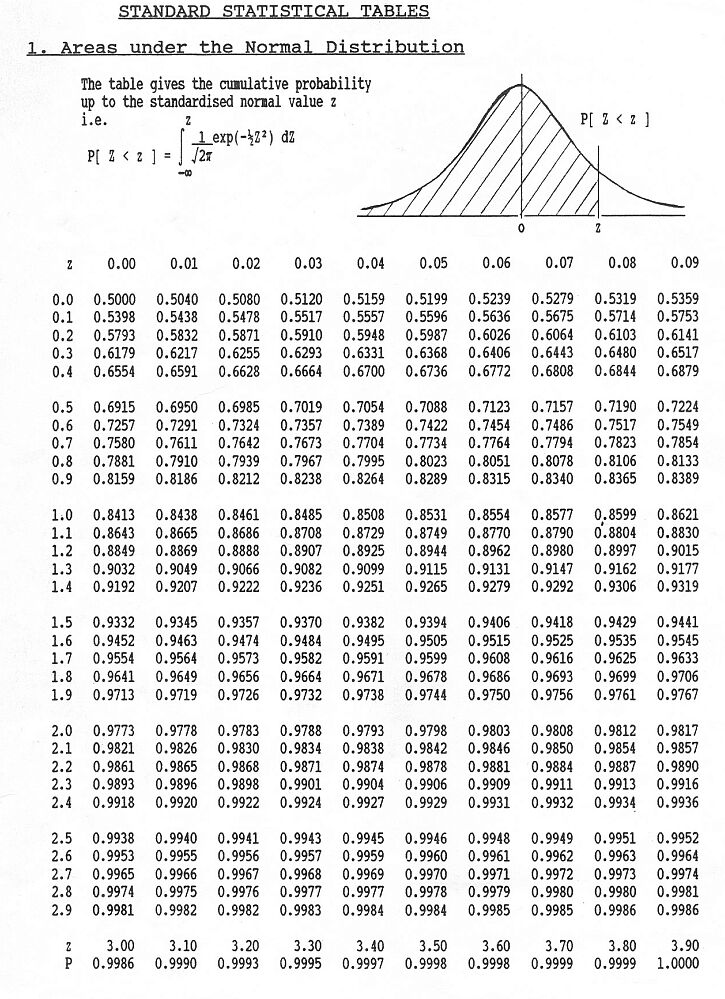
\includegraphics[width=4in]{Normal01.jpg}
\end{figure}


}


\frame{ \frametitle{Standardization}

Recall, a \textbf{standard} random variable has mean 0 and variance 1. 

\vspace{3mm}

For a random variable $X$ with mean $E(X) = \mu$ and variance $Var(X) = \sigma^2$, the \textbf{standardized} version of $X$ is 
\[ Z = \frac{X - \mu}{\sigma}. \]
We use this transformation often in discussing normal random variables, to turn questions about probabilities for $X$ into probabilities for $Z$ (which can then be read off the $Z$-table). 

}


\frame{ \frametitle{Problems involving the normal distribution}

Let $X \sim N(\mu, \sigma^2)$ and $Z \sim N(0,1)$. \\

\vspace{3mm}

Then $X \sim \sigma Z + \mu$ and $Z \sim \frac{X - \mu}{\sigma}$. 

\vspace{3mm}

What is $P(a < X < b)$?
\begin{align*} 
P(a < X < b) & = P\left( \frac{a - \mu}{\sigma} < \frac{X - \mu}{\sigma} < \frac{b - \mu}{\sigma}\right) \\
 & = P\left( \frac{a - \mu}{\sigma} < Z < \frac{b - \mu}{\sigma}\right) \\
 & = N\left( \frac{b - \mu}{\sigma} \right) - N\left( \frac{a - \mu}{\sigma}\right).
\end{align*}

}



\frame{ \frametitle{Example: IQ}

A so-called ``intelligence quotient'' (IQ) is a number scored by a variety of tests involving brainteasers, vocabulary questions, analogies, visual puzzles, and similar types of questions.  

\vspace{5mm}

Assume IQ from a particular test is normally distributed, with mean 100 and standard deviation 15.\footnote{This is a standard model construction for this kind of test: a number of people will be tested, and the test-writers will build the scoring system based on $N(100,15^2)$ as a target distribution.}

\vspace{5mm}

A certain society requires its members score in the 98th percentile on this test for entry. 

\vspace{5mm}

What is the minimum score needed on this test to enter the society?

}


\frame{ \frametitle{Example: IQ, percentile}

Let $Y$ be the IQ (from this test) of a randomly-selected test-taker. Then, assuming $Y \sim N(100, 15^2)$, we need to find $a = Q_Y(0.98)$ that gives $F_Y(a) = 0.98$. 

\vspace{5mm}

This means working backwards on the $Z$-table: find the $Z$-score associated to a CDF probability of 0.98 on the $Z$-table, and finding $a$ from there.
\begin{align*} 
& & F_Y(a) = P(Y \leq a) & = 0.98 \\
& \implies & P\left(\frac{Y - 100}{15} \leq \frac{a - 100}{15}\right) & = 0.98 \,\,\, \left(\frac{Y - 100}{15} \sim Z \sim N(0,1)\right) \\
& \implies &  P\left(Z \leq \frac{a - 100}{15}\right) & = 0.98  \,\,\, \left(\text{look up 0.98 inside Z-table}\right)\\
& \implies &  \frac{a - 100}{15} & \approx 2.055 \\
& \implies &  a & \approx 2.055(15) + 100 = 130.825.
\end{align*}

}


\end{document}
